\documentclass[handout]{beamer}
%\documentclass[presentation]{beamer}

\usecolortheme{Imperial}
 
\usepackage[utf8]{inputenc}
\usepackage[UKenglish]{babel}
\usepackage{booktabs}
\usepackage{caption}
\usepackage{subcaption}
\usepackage{graphicx}
\usepackage{amsmath}
\usepackage{amsfonts}
\usepackage{amssymb}
\usepackage{epstopdf}
\usepackage{pgfplots}
\usepackage{tabularx}
\usepackage{array}
\usepackage{xpatch}
\usepackage[export]{adjustbox}
\usepackage[maxcitenames=2, backend=biber, dashed=false, style=imperialharvard]{biblatex}
    \addbibresource{../../Write-Up/CMEE_Thesis.bib}
    \setlength\bibitemsep{0.5\baselineskip}
\renewbibmacro*{textcite}{%
  \ifnameundef{labelname}
    {\iffieldundef{shorthand}
       {\usebibmacro{cite:label}%
        \setunit{%
          \global\booltrue{cbx:parens}%
          \addspace\bibopenparen}%
        \ifnumequal{\value{citecount}}{1}
          {\usebibmacro{prenote}}
          {}%
        \usebibmacro{cite:labelyear+extrayear}}
       {\usebibmacro{cite:shorthand}}}
    {\printnames{labelname}%
     \setunit{%
       \global\booltrue{cbx:parens}%
       \addspace\bibopenparen}%
     \ifnumequal{\value{citecount}}{1}
       {\usebibmacro{prenote}}
       {}%
     \usebibmacro{citeyear}}}
    % \renewcommand*\finalnamedelim{\addspace\&\space}

% Force \textit{et al}. to be italicised

    \xpatchbibmacro{name:andothers}{%
        \bibstring{andothers}%
    }{%
    \bibstring[\emph]{andothers}%
    }
    \xpatchbibmacro{Name}{%
        \bibstring{name}
    }{%
    \bibstring[\textbf]{name}%
    }{}{} % leave these empty arguments here, seem to cause issues when ommited
    \xpatchbibmacro{textcite} % combine same author different year citations
  {\setunit{\addcomma}\usebibmacro{cite:extrayear}}
  {\setunit{\compcitedelim}\usebibmacro{cite:labelyear+extrayear}}
  {}
  {}
% Kill "Accessed on" lines in bibliography
\AtEveryBibitem{
    \clearfield{urlyear}
    \clearfield{urlmonth}
    \clearfield{doi}
    \clearfield{url}
    \clearfield{eprint}
    \clearfield{eprinttype}
}
\newcommand{\putat}[3]{\begin{picture}(0,0)(0,0)\put(#1,#2){#3}\end{picture}}
% complying UK date format, i.e. 1 January 2001
\usepackage{datetime}
\let\dateUKenglish\relax
\newdateformat{dateUKenglish}{\THEDAY~\monthname[\THEMONTH] \THEYEAR}
% \usepackage{eso-pic}
% \newcommand\AtPagemyUpperLeft[1]{\AtPageLowerLeft{%
% \put(\LenToUnit{0.9\paperwidth},\LenToUnit{0.9\paperheight}){#1}}}
% \AddToShipoutPictureFG{
%   \AtPagemyUpperLeft{{\includegraphics[width=.5cm,keepaspectratio]{./Figures/fish.png}}}
% }%
% Imperial College Logo, not to be changed!
\institute{\includegraphics[height=0.7cm]{logo.png}}

% -----------------------------------------------------------------------------




%Information to be included in the title page:
\title{Realistic Intake Rate Scaling Predicts Hyperallometric Fecundity Rate and Later Maturity In Fish}

\subtitle{Theoretical Ecology}

\author{Luke Vassor \\ \textit{M.Sc. Computational Methods in Ecology \& Evolution}}

\date{\today}



\begin{document}
 
\frame{\titlepage}


\begin{frame}
	\frametitle{Ontogenetic Growth}
	\begin{itemize}
		\item Organisms acquire resources from the environment to grow new biomass
		\item Costs to address: maintaining cells, reproduction
		\item Ecological Metabolic Theory: Growth rate slows because as we grow larger, we need to maintain more and more cells
		\item Energy intake and maintenance scale with mass differently
	\end{itemize}
	\centering
	\includegraphics[height=1cm]{./Figures/fish.png}\hspace{0.8cm}\includegraphics[height=1.5cm]{./Figures/fish.png}\hspace{0.8cm}\includegraphics[height=2cm]{./Figures/fish_fecund.png}
\end{frame}


\begin{frame}
	\frametitle{Power laws}
	\putat{-20}{-15}{\includegraphics[height=2.5cm]{./Figures/energy_flow.pdf}}
		\centering
		\begin{figure}
			\includegraphics[width=\textwidth]{./Figures/presentation_growth_schedules.pdf} \
			% remove the 'draft' keyword, when replacing with final figure!
			\caption{Maintenance (metabolic) rate scales with mass more steeply than intake rate, causing growth to slow or terminate. \\ IG = Indeterminate Grower. DG = Determinate Grower.}
		\end{figure}
\end{frame}
\begin{frame}[t]
	\frametitle{Power laws}
	\begin{columns}[t]
		\column{0.0125\textwidth}
		\column{0.4875\textwidth}
		\vspace{-0.5cm}
			\centering
			\begin{figure}
				\includegraphics[width=\textwidth]{./Figures/new_costs.pdf} \
				% remove the 'draft' keyword, when replacing with final figure!
				\caption{Introduction of new costs}
			\end{figure}
		\column{0.4875\textwidth}
			\begin{itemize}
				\item Intake rate may scale steeper
				\item Fecundity rate makes costs scale steeper
			\end{itemize}
			\begin{figure}
				\includegraphics[height=2.7cm]{./Figures/energy_flow_fecundity.pdf}				
			\end{figure}
		\column{0.0125\textwidth}
	\end{columns}
		
\end{frame}

\begin{frame}
	\frametitle{Power laws: Fecundity Rate}
	\putat{215}{-5}{\includegraphics[height=2cm]{./Figures/fish_fecund.png}}
	\begin{itemize}\setlength\itemsep{0.3cm}
		\item New results from \textcite{Barneche2018-reproductive_output}: fish fecundity output scales hyperallometrically 
		\item Bigger fish mothers are disproportionately more fecund - but only a snapshot
	\end{itemize}
	\centering
				\begin{figure}
					\includegraphics[height=3cm]{{./Figures/diego_hyperallometry}.pdf} \
					% remove the 'draft' keyword, when replacing with final figure!
					\caption{95\% species showed hyperallometric fecundity output}
				\end{figure}
\end{frame}

\begin{frame}
	\frametitle{Aims}
	\begin{columns}[t]
		\column{0.0125\textwidth}
		\column{0.4875\textwidth}
		\begin{block}{Biphasic Growth model}
			\begin{align*}
				\frac{dm}{dt} &= am^{0.75} - bm \\ %\ \ \ \ \ \ \ m < m_{\alpha}\\
				\frac{dm}{dt} &= am^{0.75} - bm - cm^{\rho} \\ %\ \ \ \ \  \ \ \ m \geq m_{\alpha}
				R_0 &= \int_{\alpha}^{\infty}l(t)cm^{\rho}h(t) dt
			\end{align*}
		\end{block}
		
		\column{0.4875\textwidth}
		\centering
		\begin{figure}
			\includegraphics[width=\textwidth]{../../Results/single_curve_with_onset.pdf}   \
				% remove the 'draft' keyword, when replacing with final figure!
			\caption{Example growth curve with maturity age $\alpha = 200$ days}
		\end{figure}
		\column{0.0125\textwidth}
	\end{columns}
	\begin{itemize}\setlength\itemsep{0.3cm}
		\item Simulate variable $c$ and $\rho$ - does hyperallometry emerge?
		\item How does intake rate scaling affect the likelihood of this?
	\end{itemize}
\end{frame}

\begin{frame}
	\frametitle{Results - Varying Intake Rate Scaling}
	\begin{columns}[b]
		\column{0.0125\textwidth}
		\column{0.4875\textwidth}
			\centering
			\begin{figure}
				\includegraphics[width=\textwidth]{{../../Results/opt_hm_Alph=200.00_a=2.15_x=0.75_k=0.01_regfont}.pdf} \
				% remove the 'draft' keyword, when replacing with final figure!
				\caption{Optimum fecundity rate parameters $c,\rho$ when \textbf{intake rate scaling = 0.75}}
			\end{figure}
		\column{0.4875\textwidth}
			\centering
			\begin{figure}
				\includegraphics[width=\textwidth]{{../../Results/opt_hm_Alph=200.00_a=2.15_x=0.85_k=0.01_regfont}.pdf} \
				% remove the 'draft' keyword, when replacing with final figure!
				\caption{Optimum fecundity rate parameters $c,\rho$ when \textbf{intake rate scaling = 0.85}}
			\end{figure}
		\column{0.0125\textwidth}
	\end{columns}
\end{frame}

\begin{frame}
	\frametitle{Results - Varying Age-At-Maturity, $\alpha$}
	\begin{columns}[b]
		\column{0.0125\textwidth}
		\column{0.4875\textwidth}
			\centering
			\begin{figure}
				\includegraphics[width=\textwidth]{{../../Results/alpha_sensitivity_x=0.75}.pdf}   \
				% remove the 'draft' keyword, when replacing with final figure!
				\caption{Optimum $\rho$ for different maturity ages when \textbf{intake rate scaling of 0.75}}
			\end{figure}
		\column{0.4875\textwidth}
			\centering
			\begin{figure}
				\includegraphics[width=\textwidth]{{../../Results/alpha_sensitivity_x=0.85}.pdf}  \
				% remove the 'draft' keyword, when replacing with final figure!
				\caption{Optimum $\rho$ for different maturity ages when \textbf{intake rate scaling of 0.75}}
			\end{figure}
		\column{0.0125\textwidth}
	\end{columns}
\end{frame}

\begin{frame}
	\putat{0}{-44}{\includegraphics[height=0.5cm]{./Figures/Gadus.png}}
	\putat{0}{-75}{\includegraphics[height=0.5cm]{./Figures/salmon_chinook.jpeg}}
	\putat{-5}{-95}{\includegraphics[height=0.5cm]{./Figures/yellowtail-flounder.png}}
	\frametitle{Realistic maturity ages}
	\begin{itemize}\setlength\itemsep{0.5cm}
		\item Empirically, fish have been observed to mature after years of growth (in the order of thousands of days)
		\begin{itemize}\setlength\itemsep{0.2cm}
			\item Cod: 2-4 years \autocite{OBrien1993, Rochet2001, Knickle2013}
			\item Chinook Salmon: 2-5 years \autocite{groot1991pacific}
			\item Yellowtail flounder: 2-5 years \autocite{OBrien1993}
		\end{itemize}
		\item Maturity ages this late necessitate steeper intake rate scaling
	\end{itemize}
\end{frame}

\begin{frame}
	\frametitle{Future direction}
	\begin{itemize}\setlength\itemsep{0.5cm}
		\item ``Reverse-engineer'' consumption rate scaling from \textcite{Barneche2018-reproductive_output} data - I predict that fish species showing hyperallometric fecundity come from high intake environments
		\item Need better understanding of consumption versus intake - requires digestion efficiency data and foraging time data
		\item Collect data on and develop theory for continuous rate of fecundity allocation
	\end{itemize}
\end{frame}
\begin{frame}
	\frametitle{Acknowledgements}
	\vspace{-0.5cm}
	\begin{table}[]
		\begin{tabular}{m{9.5cm}m{5cm}}
		Dr Samraat Pawar (Primary Supervisor, Imperial College)               			& \includegraphics[height=1.2cm]{Figures/samraat.jpg} \\
		Dr Diego Barneche (Secondary Supervisor, Univ. of Exeter) 			& \includegraphics[height=1.2cm]{Figures/Diego_R_Barneche.jpg} \\
		Tom Clegg (PhD Student, Imperial College)                    					& 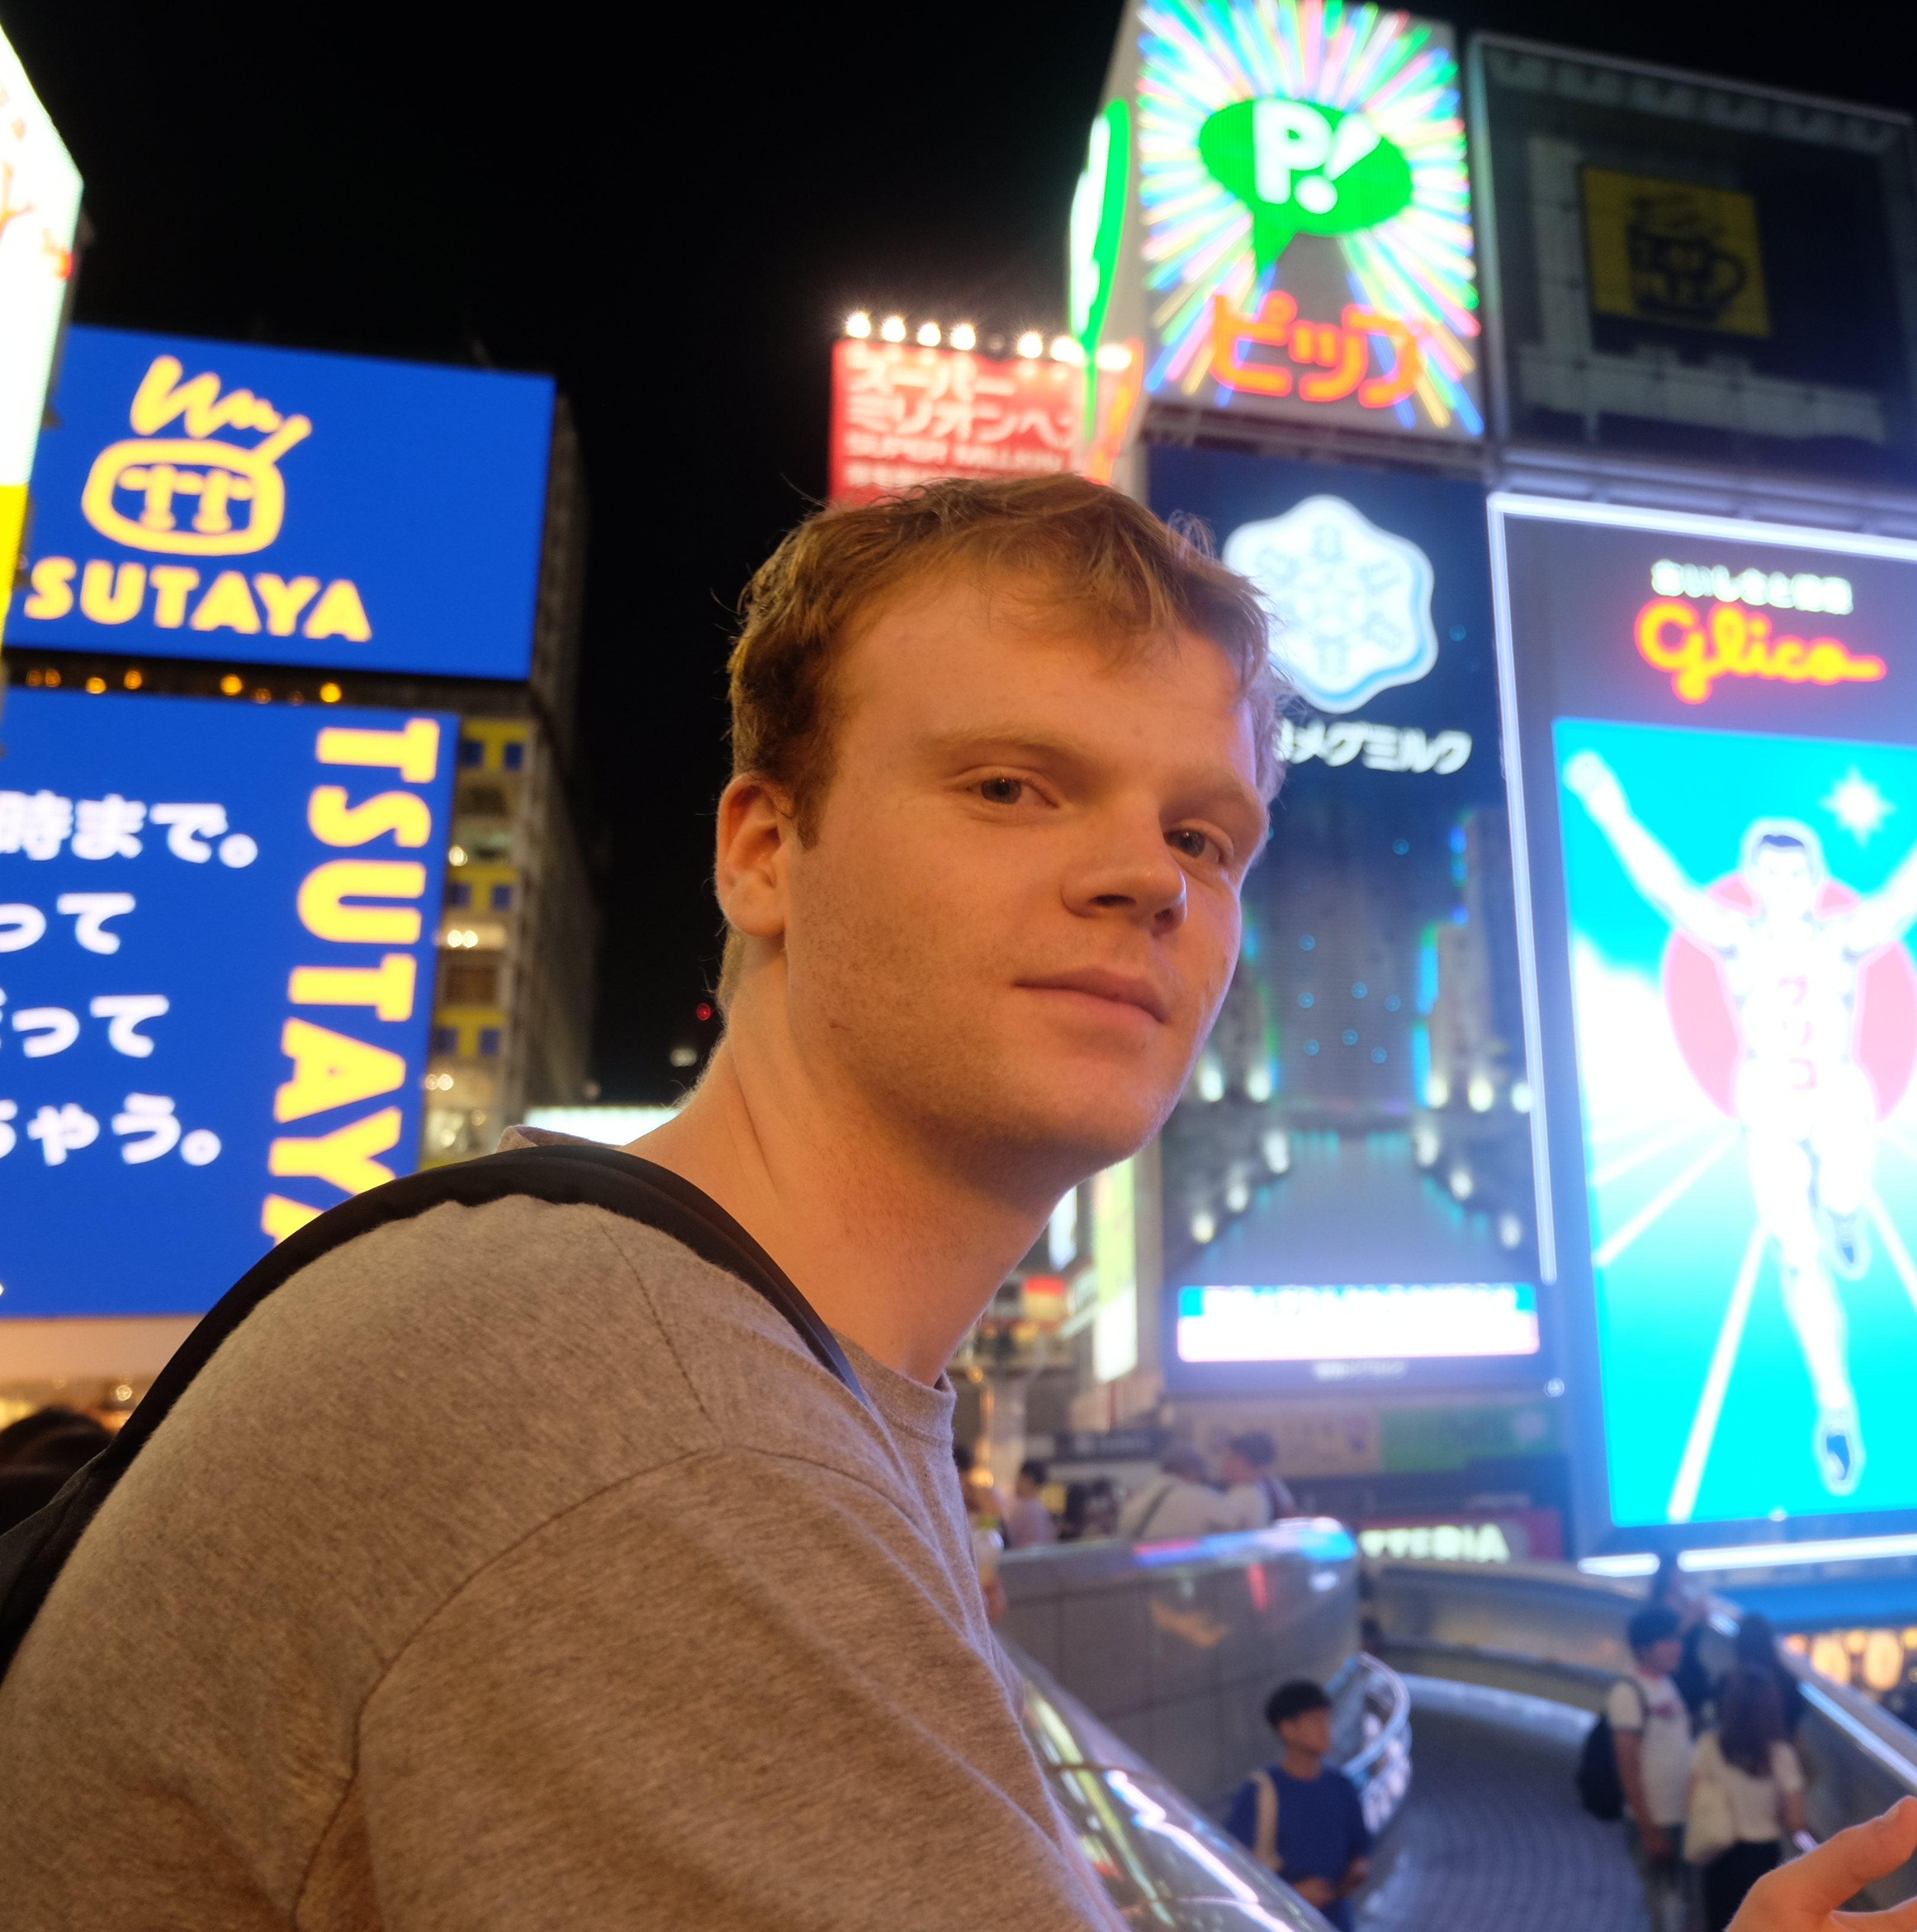
\includegraphics[height=1.2cm]{Figures/tom_clegg.JPG} \\
		Prof Van Savage (UCLA)                                        		& \includegraphics[height=1.2cm]{Figures/van_savage.jpg} \\
		Prof Dustin Marshall (Monash University, Melbourne)                     		& \includegraphics[height=1.2cm]{Figures/dustin_marshall.jpg}
		\end{tabular}
		\end{table}
\end{frame}
\end{document}